\section{The concept of feasible directions}

Feasible direction methods are a class of methods that incorporate both improvement and feasibility requirements when devising search directions. As feasibility is also observed throughout the solution process, they are also referred to as \emph{primal methods}. However, depending. on the geometry of the feasible region, it might be so that the method allow for some infeasibility in the course of the algorithm, as we will see later.

An \emph{improving feasible direction} can be defined as follows.
%
\begin{definition}
Consider the problem $\mini\braces{f(x) : x \in S}$ with $f:\reals^n \rightarrow \reals$ and $\emptyset \neq S \subseteq \reals^n$. A vector $d$ is a feasible direction at $x \in S$ if exists $\delta > 0$ such that $x + \lambda d \in S$ for all $\lambda \in (0,\delta)$. Moreover, $d$ is an improving feasible direction at $x \in S$ if there exists a $\delta > 0$ such that $f(x + \lambda d) < f(x)$ and $x + \lambda d \in S$ for $\lambda \in (0,\delta)$. 
\end{definition}
%
The key feature of feasible direction methods is the process of deriving such directions and associated step sizes that retain feasibility, even if approximately. Similarly to the other methods we have discussed in the past lectures, these methods progress following two basic steps:
\begin{enumerate}
\item Obtain an \emph{improving feasible direction} $d^k$ and a step size $\lambda^k$;
\item Make $x^{k+1} = x^k + \lambda^kd^k$.
\end{enumerate}

As a general rule, for a feasible direction method to perform satisfactorily, it must be that the calculation of the directions $d^k$ and step sizes $\lambda^k$ are simple enough. Often, these steps can be reduced to closed forms or, more frequently, solving linear or quadratic programming problems, or even from posing modified Newton systems.


\section{Conditional gradient - the Frank-Wolfe method}

The conditional gradient method is named as such due to the direction definition step, in which the direction $d$ is selected such that the angle between the gradient $\nabla f(x)$ and $d$ is as close to 180$^\circ$ degrees as the feasible region $S$ allows.

Recall that, if $\nabla f(x^k)$ is a \emph{descent direction}, then 
%
\begin{equation*}
\nabla f(x^k)^\top(x - x^k) < 0 \text{ for } x \in S.
\end{equation*}
%
A straightforward way to obtain improving feasible directions $d = (x - x^k)$ is by solving the \emph{direction search problem} $DS$ of the form
%
\begin{equation*}
(DS) : \mini ~ \braces{\nabla f(x^k)^\top (x - x^k) : x \in S}.
\end{equation*}
%

Problem $DS$ consists of finding the furtherest feasible point in the direction of the gradient, that is we move in the direction of the gradient, under condition that we stop if the line search mandates so, or that the search reach at the boundary of the feasible region. This is precisely what gives the name \emph{conditional gradient}.

By letting $\overline{x}^k = \arg\min_{x \in S} \braces{\nabla f(x^k)^\top (x - x^k)}$ and obtaining $\lambda^k \in (0,1]$ employing a line search, the method iterates making
\begin{equation*}
	x^{k+1} = x^k + \lambda^k(\overline{x}^k - x^k).
\end{equation*}
%
One important condition to observe is that $\lambda^k$ has to be constrained such that $\lambda \in (0,1]$ to guarantee feasibility, as $\overline{x}^k$ is feasible by definition. Also, notice that the condition $\nabla f(x^k) = 0$ might never be achieved, since it might be so that the unconstrained optimum is outside the feasible region $S$. In that case, after two successive iterations we will observe that $x^{k} = x^{k-1}$ and thus that $d^k=0$. This eventual stall of the algorithm will happen at a point $x^k$ satisfying first-order (constrained) optimality conditions. Therefore, the term $\nabla f(x)^\top d^k$ will become zero regardless whether the minimum of them function belongs to $S$, and is hence used as the stopping condition of the algorithm. Algorithm \ref{Alg1} summarises the Frank-Wolfe method.  

\begin{algorithm}[H]
\caption{Franke-Wolfe method} \label{Alg1}
\begin{algorithmic}[1] %line numbering frequency. 
\State {\bf initialise.} $\epsilon > 0, x^0 \in S, k = 0$. 
\While {$\nabla |f(x)^\top d^k| > \epsilon$} 
    \State $\overline{x}^k = \arg\min \braces{\nabla f(x^k)^\top d : x \in S}$ 
    \State $d^k = \overline{x}^k - x^k$
    \State $\lambda^k = \arg\min_\lambda \braces{f(x^k + \lambda d^k) : 0\leq \lambda \leq \overline{\lambda}}$
    \State $x^{k+1} = x^k + \lambda^k d^k$ 
    \State $k = k+1$
\EndWhile
\State {\bf return} $x^k$
\end{algorithmic}
\end{algorithm}
  
Notice that, for a polyhedral feasibility set, the subproblems are linear programming problems, meaning that the Frank-Wolfe method can be restarted fairly efficiently using dual simplex at each iteration. 

Figure \ref{fig:frank_wolfe} shows the employment of the FW method for optimising a nonlinear function within a polyhedral feasibility set. We consider the problem
%%
\begin{align*}
	\mini & e^{-(x_1-3)/2} + e^{(4x_2 + x_1 - 20)/10} + e^{(-4x_2 + x_1)/10}\\
	\st & 2x_1 + 3x_2 \leq 8 \\
	& x_1 + 4x_2 \leq 6,
	& x_1, x_2 \ge 0	
\end{align*}
starting from $(0,0)$ and using an exact line search to set step sizes $\lambda \in [0,1]$. Notice that the method can be utilised with inexact line searches as well. 

\begin{figure}
	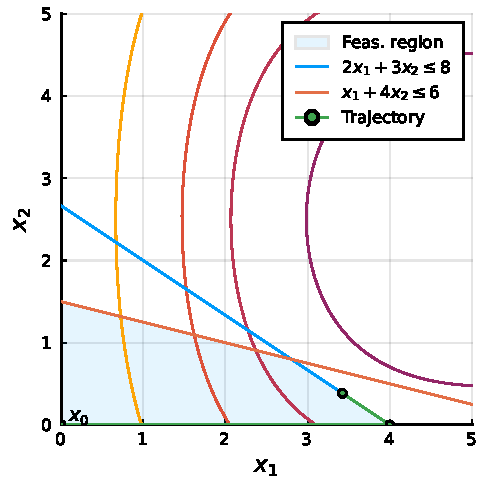
\includegraphics[width=0.49\textwidth]{part_2/chapter_11/figures/FW_alliter}
	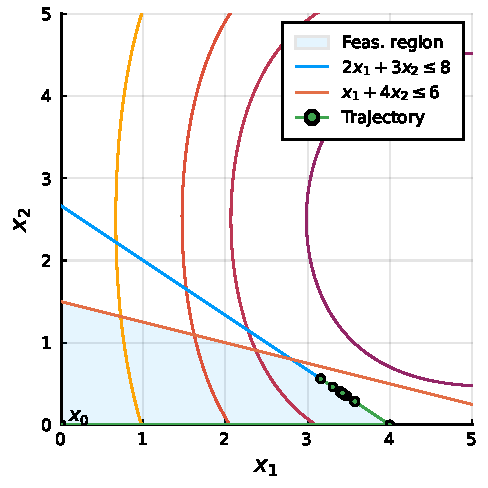
\includegraphics[width=0.49\textwidth]{part_2/chapter_11/figures/FW_alliter_armijo}	
	\caption{The Frank-Wolfe method applied to a problem with linear constraints. The algorithm takes 2 steps using an exact line search (left) and 15 with Armijo line search (right).} \label{fig:frank_wolfe}
\end{figure}

% Consider mentioning SDM as an approach.


\section{Sequential quadratic programming}


Sequential quadratic programming (SQP) is a method inspired by the idea that the KKT system of a nonlinear problem can be solved using Newton's method. It consists perhaps of the most general method in terms of considering both nonlinear constraints and nonlinear objective function. 

To see how that works, let us first consider an equality constraint problem $P$ as
$$
P = \mini\braces{f(x) : h(x) = 0, i = 1,\dots,l}.$$ 
The KKT conditions for $P$ are given by the system $W(x,v)$ where
$$
W(x,v) = \begin{cases} \nabla f(x) + \sum_{i=1}^{l}v_i\nabla h_i(x) = 0\\
                       h_i(x) = 0, \ i = 1, \dots, l  
         \end{cases}
$$
Using the Newton(-Raphson) method, we can solve $W(x,v)$. Starting from $(x^k, v^k)$, we can solve $W(x,v)$ by successively employing Newton steps of the form
%
\begin{equation} \label{eq:NewtonSystem}
W(x^k, v^k) + \nabla W(x^k, v^k)\begin{bmatrix} x - x^k\\
                                                v - v^k 
                                \end{bmatrix} = 0.
\end{equation}
%
Upon closer inspection, one can notice that the term $\nabla W(x,v)$ is given by
$$ \nabla W(x^k, v^k) = \begin{bmatrix} \nabla^2L(x^k,v^k) & \nabla h(x^k)^\top\\
                                        \nabla h(x^k)        & 0
                        \end{bmatrix},
$$
where 
$$
\nabla^2L(x^k,v^k) = \nabla^2f(x^k) + \sum_{i=1}^lv^k_i\nabla^2h_i(x^k)
$$ 
is the \emph{Hessian of the Lagrangian} function 
$$
L(x,v) = f(x) + v^\top h(x) 
$$
at $x^k$. Now, setting $d = (x - x^k)$, we can rewrite \eqref{eq:NewtonSystem} as
%
\begin{align}
& \nabla^2L(x^k,v^k)d + \nabla h(x^k)^\top v = -\nabla f(x^k) \label{QP_opt_cond1}\\
& \nabla h(x^k)d = -h(x^k), \label{QP_opt_cond2}
\end{align}
which can be repeatedly solved until 
$$
||(x^{k},v^k)^\top - (x^{k-1}, v^{k-1})^\top|| = 0,
$$
i.e., convergence, is observed. Then, $(x^{k},v^{k})$ is a KKT point by definition.

This is fundamentally the underlying idea of SQP, however the approach is taken under a more specialised setting. Instead of relying on Newton steps, we resort on successively solving quadratic subproblems of the form
%
\begin{align}
QP(x^k, v^k) : \mini \ & f(x^k)+ \nabla f(x^k)^\top d + \frac{1}{2}d^\top\nabla^2L(x^k,v^k)d \label{eq:QP_objfun}\\
\st & h_i(x^k) + \nabla h_i(x^k)^\top d = 0, i = 1,\dots,l. \label{eq:QP_const}
\end{align}
%
Notice that $QP$ is a linearly constrained quadratic programming problem, for which we have seen several solution approaches. Moreover, notice that the optimality conditions of $QP$ are given by \eqref{QP_opt_cond1} and \eqref{QP_opt_cond2}, where $v$ is the dual variable associated with the constraints in \eqref{eq:QP_const}, which, in turn, represent first-order approximations of the original constraints. 

The objective function in $QP$ can be interpreted as being a second-order approximation of $f(x)$ enhanced with the term $(1/2)\sum_{i=1}^lv^k_id^\top\nabla^2 h_i(x^k)d$ that captures constraint curvature information. 

An alternative interpretation for the objective function of $QP$ is to notice that it consists of the second order approximation of the Lagrangian function $L(x,v) = f(x) + \sum_{i=1}^lv_ih_i(x)$ at $(x^k, v^k)$, which is given by 
%
\begin{align*}
	L(x,v) &\approx L(x^k,v^k) + \nabla_{x}L(x^k, v^k)^\top d + \frac{1}{2}d^\top \nabla^2L(x^k,v^k)d \\	
		   &= f(x_k) + {v^k}^\top h(x^k) + (\nabla f(x^k) + {v^k}^\top \nabla h(x^k))^\top d + \frac{1}{2}d^\top (\nabla^2f(x^k) + \sum_{i=1}^lv^k_i\nabla^2h_i(x^k))d 
\end{align*}
% 
To see this, notice that terms $f(x^k)$, $v^{k\top}h(x^k)$ are constants and that $\nabla h(x^k)^\top (x - x^k) = 0$ (from \eqref{eq:QP_const}, as $h(x^k) = 0$). 

The general subproblem in the SQP method can be stated as 
%
\begin{align*}
QP(x^k, u^k, v^k) : \mini \ & \nabla f(x^k)^\top d + \frac{1}{2}d^\top\nabla^2L(x^k,u^k,v^k)d \\
\st & g_i(x^k) + \nabla g_i(x^k)^\top d \leq 0, i = 1,\dots,m \\ 
& h_i(x^k) + \nabla h_i(x^k)^\top d = 0, i = 1,\dots,l,
\end{align*}
which includes inequality constraints $g_i(x) \leq 0 $ for $i=1,\dots,m$ in a linearised from and their respective associated Lagrangian multipliers $u_i$, for $i=1,\dots,m$. This is possible since we are using an optimisation setting rather than a Newton system that only allows for equality constraints, even though the latter can be obtained by simply introducing slack variables. Clearly, there are several option that could be considered to handle this quadratic problem, including employing a primal/dual interior point method.

A pseudocode for the standard SQP  method is presented in Algorithm \ref{Alg2}.

\captionsetup[algorithm]{font=footnotesize}
\begin{algorithm}[H]
\caption{SQP method} \label{Alg2}
\begin{algorithmic}[1] %line numbering frequency. 
	\State {\bf initialise.} $\epsilon > 0, x^0 \in S, u^0 \geq0, v^0, k = 0$. 
	\While {$||d^k|| > \epsilon$} 
	    \State $d^k = \arg\min QP(x^k, u^k, v^k)$
%	    \State $d^k = \overline{x}^k - x^k$
		\State obtain $u^{k+1}, v^{k+1}$ from $QP(x^k, u^k, v^k)$ \label{alg2:dual_var}
	    \State $x^{k+1} = x^k + d^k,  k = k+1$.
	\EndWhile
	\State {\bf return} $x^k$.
\end{algorithmic}
\end{algorithm}
Notice that in Line \ref{alg2:dual_var}, dual variable values are retrieved from the constraints in $QP(x^k, u^k, v^k)$. therefore, $QP(x^k, u^k, v^k)$ needs to be solved by an algorithm that can return these dual variables, such as the (dual) simplex method. 

Figure \ref{fig:sqp_example} illustrates the behaviour of the SQP method on the problem. Notice how the trajectory might eventually become infeasible due to the consideration of linear approximations of the nonlinear constraint. 

$$
\mini\braces{2x_1^2 + 2x_2^2 - 2x_1x_2 - 4x_1 - 6x_2 : x_1^2 - x_2 \leq 0, x_1 + 5x_2 \leq 5, x_1 \geq 0, x_2 \geq 0}
$$
\begin{figure}
	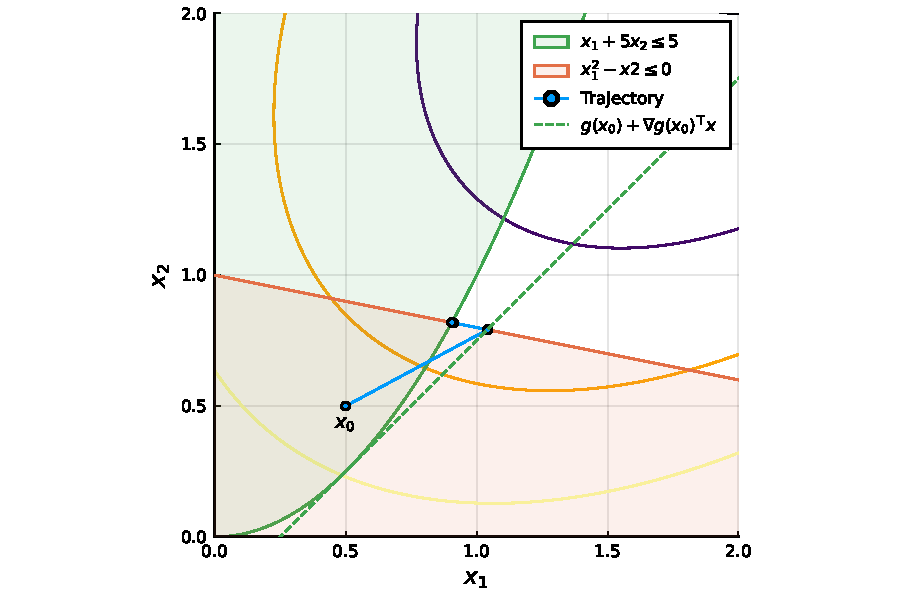
\includegraphics[width=\textwidth]{part_2/chapter_11/figures/SQP_example.pdf}
	\caption{The SQP method converges in 6 iterations with $\epsilon = 10^{-6}$} \label{fig:sqp_example}		
\end{figure}


One important feature for the SQP method is that it closely mimics the convergence properties of Newton's method and therefore, under appropriate conditions, superlinear convergence can be observed. Moreover, the BFGS method can be used to approximate $\nabla^2L(x^k,v^k)$, which can turn the method dependent only on first order derivatives.

Notice that, because the constraints are considered implicitly in the subproblem $QP(x^k, u^k, v^k)$, one cannot devise a line search for the method, which in turn, being based on successive quadratic approximations, presents a risk for divergence.

The $l_1$-SQP is a modern variant of SQP that addresses divergence issues arising in the SQP method when considering solutions that are far away from the optimum, while presenting superior computational performance. 

In essence, $l_1$-SQP relies on a similar principle than penalty methods, encoding penalisation for infeasibility in the objective function of the quadratic subproblem. In the context of SQP algorithms, these functions are called ``merit'' functions. This not only allow for considering line searches (since feasibility becomes encoded in the objective function with feasibility guaranteed at a minimum. cf. penalty methods) or, alternatively, relying on a trust region approach, ultimately preventing divergence issues.

Let us consider the trust-region based $l_1$-penalty $QP$ subproblem, which can be formulated as
%
\begin{align*}
l_1-QP&(x^k, v^k) :\\
\mini & \ \nabla f(x^k)^\top d + \frac{1}{2}d^\top\nabla^2L(x^k,v^k)d \\ & + \mu\left[ \sum_{i=1}^m [g_i(x^k) + \nabla g_i(x^k)^\top d]^+  + \sum_{i=1}^l |h_i(x^k) + \nabla h_i(x^k)^\top d| \right] \\
 \st & -\Delta^k \leq d \leq \Delta^k,  
\end{align*}
where $\mu$ is a penalty term, $[\, \cdot \,] = \max\braces{0, \cdot}$, and $\Delta^k$ is a trust region term. This variant is of particular interest, because the subproblem $l_1-QP(x^k, v^k) $ can be recast as a QP problem with linear constraints:
%
\begin{align*}
l_1-QP&(x^k, v^k) :\\
\mini & \ \nabla f(x^k)^\top d + \frac{1}{2}d^\top\nabla^2L(x^k,v^k)d  + \mu\left[ \sum_{i=1}^m y_i  + \sum_{i=1}^l (z^+_i - z^-_i) \right]\\
 \st & -\Delta^k \leq d \leq \Delta^k\\
 & y_i \geq g_i(x^k) + \nabla g_i(x^k)^\top d, i = 1\dots, m\\
 & z^+_i - z^-_i = h_i(x^k) + \nabla h_i(x^k)^\top d, i = 1,\dots,l \\ 
 &y, z^+, z^- \geq 0.   
\end{align*}
%
The subproblem $l_1-QP(x^k, v^k)$ enjoys the same benefits the original form, meaning that it can be solved with efficient simplex-method based solvers. 

The trust-region variant of $l_1$-SQP is globally convergent (does not diverge) and enjoys superlinear convergence rate, as the original SQP. The $l_1$-penalty term is what is often called a \emph{merit function} in the literature. Alternatively, one can disregard the trust region and employ a line search (either exact or inexact) which would also enjoy globally convergent properties.  


\section{Generalised reduced gradient*}


The generalised reduced gradient method resembles in many aspects the simplex method for linear optimisation problems. It derives from the Wolfe's reduced gradient. The term ``reduced'' refers to the consideration of a reduced variable space, formed by a subset of the decision variables.

\subsection{Wolfe's reduced gradient}

Let us consider the linearly constrained problem:
\begin{flalign*}
(P) ~:~ \mini \ & f(x) \\
\st & Ax = b \\
& Ax \geq 0, 
\end{flalign*}
where $f : \reals^n \rightarrow \reals$ is differentiable, $A$ is $m \times n$ and $b \in \reals^m$.

To ease the illustration, we assume linear programming \emph{nondegeneracy}, i.e., that any $m$ columns of $A$ are linearly independent and every extreme point of feasible region has at least $m$ positive components and at most $n-m$ zero components.

Being so, let us define a partition of $A$ as $A = (B, N)$, $x^\top = (x_B^\top, x_N^\top)$, where $B$ is an invertible $m \times m$ matrix with $x_B > 0$ as a basic vector and $x_N \geq 0$ as a nonbasic vector. This implies that $\nabla f(x)^\top$ can also be partitioned as $\nabla f(x)^\top= (\nabla_Bf (x)^\top, \nabla_Nf(x)^\top)$.

In this context, for $d$ to be an improving feasible direction, we must observe that
\begin{enumerate}
	\item $\nabla f(x)^\top d < 0$
	\item $Ad = 0$, with $d_j \geq 0$ if $x_j = 0$ to retain feasibility.  
\end{enumerate}

We will show how to obtain a direction $d$ that satisfies conditions 1 and 2. For that, let $d^\top = (d_B^\top, d_N^\top)$. We have that $0 = Ad = Bd_B + Nd_n$ for any $d_N$, implying that $d_B = -B^{-1}Nd_N$. Moreover,
\begin{align}
	\nabla f(x)^\top d & = \nabla_B f(x)^\top d_B + \nabla_N f(x)^\top d_N \nonumber\\
	& = (\nabla_N f(x)^\top - \nabla_Bf(x)^\top B^{-1}N)d_N \label{eq:red_grad}
\end{align}

The term $r_N^\top = (\nabla_N f(x)^\top - \nabla_Bf(x)^\top B^{-1}N)$ is referred to as the reduced gradient as it express the gradient of the function in terms of the nonbasic directions only. Notice that the reduced gradient $r$ holds a resemblance to the reduced costs from the simplex method. In fact
%
\begin{align*}
	r^\top & =  (r_B^\top, r_N^\top) = \nabla f(x) - \nabla_Bf(x)^\top B^{-1}A \\ 
 	& =  (\nabla_B f(x) - \nabla_B f(x)^\top B^{-1}B, \nabla_N f(x) - \nabla_B f(x)^\top B^{-1}N) \\
 	& = (0, \nabla_N f(x) - \nabla_B f(x)^\top B^{-1}N),
\end{align*}
%
and thus $\nabla f(x) = r^\top d$.

Therefore, $d_N$ must be chosen such that $r_N^\top d_N < 0$ and $d_j \geq 0$ if $x_j = 0$. One way of achieving so is employing the classic \emph{Wolfe's rule}, which states that
$$d_j = \begin{cases} -r_j, \text{ if } r_j \leq 0, \\
                      -x_jr_j, \text{ if } r_j > 0.
        \end{cases}
$$ 
Notice that the rule is related with the direction of the optimisation. For $r_j \leq 0$, one wants to increase the value of $x_j$ in that coordinate direction, making $d_j$ non-negative. On the other hand, if the reduced gradient is positive ($r_j > 0$), one wants to reduce the value of $x_j$, unless it is already zero, a safeguard created by multiplying $x_j$ in the definition of the direction $d$.

The following result guarantee the convergence of Wolfe's reduced gradient to a KKT point.
%
\begin{theorem}
Let $\overline{x}$ be a feasible solution to $P$ such that $\overline{x} = (\overline{x}_B^\top, \overline{x}_N^\top)$ and $x_B > 0$. 
Consider that $A$ is decomposed accordingly into $(B,N)$. Let $r^\top = \nabla f(\overline{x})^\top - \nabla_B f(\overline{x})^\top B^{-1}A$ and let $d$ be formed using Wolfe's rule. Then
\begin{enumerate}
\item if $d \neq 0$, then $d$ is an improving direction;
\item if $d = 0$, then $\overline{x}$ is a KKT point.
\end{enumerate}
\end{theorem}
%
\begin{proof}
$d$ is a feasible direction by construction. Now, notice that 
\begin{align*}
\nabla f(\overline{x}) ^\top d &= \nabla_B f(\overline{x})^\top d_B + \nabla_N f(\overline{x})^\top d_N \\
& = [\nabla_N f(\overline{x})^\top - \nabla_B f(\overline{x})^\top B^{-1}N]d_N = \sum_{j \notin I_B}r_jd_j
\end{align*}
where $I_B$ is the index set of basic variables. By construction (using Wolfe's rule), either $d=0$ or $\nabla f(\overline{x})^\top d < 0$, being thus an \emph{improvement direction}.

$\overline{x}$ is a KKT point if and only if there exists $(u_B^\top, u_N^\top) \geq (0, 0)$ and $v$ such that
\begin{align}
&(\nabla_B f(x)^\top, \nabla_N f (x)^\top) + v^\top(B,N) - (u_B^\top, u_N^\top) = (0,0) \label{eq:firstKKT}\\
&u_B^\top x_B = 0, u_N^\top x_N = 0. \label{eq:secondKKT}
\end{align}

Since $x_B > 0$ and $u_B \geq 0$, $u_B^\top x_B = 0$ if and only if $u_B = 0$. From top row in \eqref{eq:firstKKT}, $v^\top = -\nabla_Bf(x)B^{-1}$. Substituting in the bottom row of \eqref{eq:firstKKT}, we obtain $u_N^\top = \nabla_N f(x)^\top - \nabla_B f(x)^\top B^{-1}N = r_N$.

Thus, the KKT conditions reduce to $r_N \geq 0$ and $r_N^\top x_N = 0$, only observed when $d = 0$ by definition.
\end{proof}

Algorithm \ref{Alg3} presents a pseudocode for the Wolfe's reduced gradient. A few implementation details stand out. First, notice that the basis is selected choosing the largest components in value, which differs from the simplex method by allowing for nonbasic variables to assume nonzero values. Moreover, notice that a line search is employed conditioned on bounds on the step size $\lambda$ to guarantee that feasibility $x \geq 0 $ is retained. 

\begin{algorithm}[H]
\caption{Wolfe's reduced gradient method} \label{Alg3}
\begin{algorithmic}[1] %line numbering frequency. 
\State {\bf initialise.} $\epsilon > 0, x^0 \text{ with } Ax^k = b, k = 0$, columns $a_j$, $j = 1, \dots, n$ of $A$  
\While {$||d^k|| > \epsilon$} 
    \State $I^k = $ index set for $m$ largest components of $x^k$
    \State Let $A = (B, N)$, where $B = \braces{a_j : j \in I^k}$, and $N = \braces{a_j : j \notin I^k}$
    \State $r^{k\top} = \nabla f(x^k)^\top - \nabla_B f(x^k)^\top B^{-1}A$
    \State $d^k_j = \begin{cases} -r^k_j, \text{ if } j \notin I^k \text{ and } r_j \leq 0; \\
                                  -r_jx_j, \text{ if } j \notin I^k { and } r_j > 0.   
                            \end{cases}$
     \State $d_B = - B^{-1}Nd_N$
     \If {$d = 0$}
         \State {\bf return} $x^k$
     \EndIf
    \State $\overline{\lambda} = \begin{cases} +\infty, \text{ if } d^k \geq 0; \\
                                          \min\braces{x_j^k/d_j^k :  d_j^k < 0}, \text{ if } d^k < 0.   
                            \end{cases}$                                
    \State $\lambda^k = \arg\min \braces{f(x^k + \lambda d^k) : 0\leq \lambda \leq \overline{\lambda}}$.
    \State $x^{k+1} = x^k + \lambda^k d^k; k = k+1$.
\EndWhile
\State {\bf return} $x^k$.
\end{algorithmic}
\end{algorithm}
  
\subsection{Generalised reduced gradient method}

The \emph{generalised reduced gradient} extends Wolfe's method by:
\begin{enumerate}
\item Nonlinear constraints are considered via first-order approximation at $x^k$
$$h(x^k) + \nabla h(x^k) ^\top(x - x^k) = 0 \Rightarrow h(x^k) ^\top x =  h(x^k)^\top x^k.
$$
with an additional \emph{restoration phase} that has the purpose of recovering feasibility via projection or using Newton's method.
\item Consideration of \emph{superbasic variables}. In that, $x_N$ is further partitioned into $x_N^\top = (x_S^\top, x_{N'}^\top)$. 
\end{enumerate}

The superbasic variables $x_S$ (with index set $J_S$, $0 \leq |J_S| \leq n-m$), are allowed change value, while $x_{N'}$ are kept at their current value. Hence, $d^\top = (d_B^\top, d_S^\top, d_{N'}^\top)$, with $d_{N'} = 0$. From $Ad = 0$, we obtain $d_B = -B^{-1}Sd_S$. Thus $d$ becomes
$$d = \begin{bmatrix} d_B \\ d_S \\ d_{N'}
 
      \end{bmatrix} = 
      \begin{bmatrix} -B^{-1}S \\ I \\ 0
      
      \end{bmatrix}d_S. 
$$
